% =============================================================================
% Lecture 10: Neural Networks — LSTM and Attention for Business Forecasting
% BSAD 8310: Business Forecasting | University of Nebraska at Omaha
% =============================================================================
\documentclass[aspectratio=169, 10pt]{beamer}
% =============================================================================
% header.tex — BSAD 8310: Business Forecasting
% University of Nebraska at Omaha
% Beamer theme: UNO-branded, clean, professional
% =============================================================================

% ----------------------------- BEAMER THEME ----------------------------------
\usetheme{default}
\useinnertheme{rectangles}

% ----------------------------- UNO COLOR PALETTE -----------------------------
\definecolor{unoblue}{HTML}{005CA9}
\definecolor{unored}{HTML}{E41C38}
\definecolor{unogray}{HTML}{525252}
\definecolor{unogreen}{HTML}{15803d}
\definecolor{unolightblue}{HTML}{E8F0FA}
\definecolor{unolightred}{HTML}{FDECEA}
\definecolor{unolightgreen}{HTML}{F0FAF4}
\definecolor{unowhite}{HTML}{FFFFFF}

% Apply UNO colors to Beamer structure
\setbeamercolor{structure}{fg=unoblue}
\setbeamercolor{palette primary}{bg=unoblue, fg=white}
\setbeamercolor{palette secondary}{bg=unoblue!80!black, fg=white}
\setbeamercolor{palette tertiary}{bg=unoblue!60!black, fg=white}
\setbeamercolor{frametitle}{bg=unoblue, fg=white}
\setbeamercolor{frametitle right}{bg=unoblue!80!black}
\setbeamercolor{title}{fg=unoblue}
\setbeamercolor{subtitle}{fg=unogray}
\setbeamercolor{author in head/foot}{bg=unoblue, fg=white}
\setbeamercolor{title in head/foot}{bg=unoblue!80, fg=white}
\setbeamercolor{date in head/foot}{bg=unoblue!60, fg=white}
\setbeamercolor{page number in head/foot}{bg=unoblue!60, fg=white}
\setbeamercolor{block title}{bg=unoblue, fg=white}
\setbeamercolor{block body}{bg=unolightblue}
\setbeamercolor{block title alerted}{bg=unored, fg=white}
\setbeamercolor{block body alerted}{bg=unolightred}
\setbeamercolor{block title example}{bg=unogreen, fg=white}
\setbeamercolor{block body example}{bg=unolightgreen}
\setbeamercolor{itemize item}{fg=unoblue}
\setbeamercolor{itemize subitem}{fg=unored}
\setbeamercolor{enumerate item}{fg=unoblue}
\setbeamercolor{enumerate subitem}{fg=unored}
\setbeamercolor{alerted text}{fg=unored}

% ----------------------------- FONTS -----------------------------------------
\usefonttheme{professionalfonts}
\usefonttheme[onlymath]{serif}       % serif math; sans-serif text
\setbeamerfont{frametitle}{size=\large, series=\bfseries}
\setbeamerfont{title}{size=\LARGE, series=\bfseries}
\setbeamerfont{subtitle}{size=\large}
\setbeamerfont{block title}{size=\normalsize, series=\bfseries}
\setbeamerfont{footline}{size=\tiny}

% ----------------------------- LAYOUT ----------------------------------------
\setbeamersize{text margin left=0.5cm, text margin right=0.5cm}
\setbeamertemplate{navigation symbols}{}   % remove navigation buttons
\setbeamertemplate{itemize items}[circle]
\setbeamertemplate{enumerate items}[default]

% Custom footline: [Course] [Title] [Page/Total]
\setbeamertemplate{footline}{%
  \leavevmode%
  \hbox{%
    \begin{beamercolorbox}[wd=.33\paperwidth, ht=2.5ex, dp=1ex, left, leftskip=4pt]
      {author in head/foot}%
      \usebeamerfont{author in head/foot}\insertshortauthor
    \end{beamercolorbox}%
    \begin{beamercolorbox}[wd=.34\paperwidth, ht=2.5ex, dp=1ex, center]
      {title in head/foot}%
      \usebeamerfont{title in head/foot}\insertshorttitle
    \end{beamercolorbox}%
    \begin{beamercolorbox}[wd=.33\paperwidth, ht=2.5ex, dp=1ex, right, rightskip=4pt]
      {date in head/foot}%
      \usebeamerfont{date in head/foot}%
      \insertframenumber{} / \inserttotalframenumber
    \end{beamercolorbox}%
  }%
  \vskip0pt%
}

% Frametitle with thin accent line
\setbeamertemplate{frametitle}{%
  \vskip0.1cm
  \insertframetitle
  \vskip0.05cm
  \color{unored}\rule{\textwidth}{0.5pt}
}

% Title page
\setbeamertemplate{title page}{%
  \vfill
  \begin{center}
    {\color{unoblue}\rule{\textwidth}{2pt}}\\[0.3cm]
    {\usebeamerfont{title}\usebeamercolor[fg]{title}\inserttitle}\\[0.2cm]
    {\usebeamerfont{subtitle}\usebeamercolor[fg]{subtitle}\insertsubtitle}\\[0.3cm]
    {\color{unored}\rule{\textwidth}{0.5pt}}\\[0.4cm]
    {\small\insertauthor}\\[0.1cm]
    {\small\insertinstitute}\\[0.1cm]
    {\small\insertdate}
  \end{center}
  \vfill
}

% ----------------------------- PACKAGES --------------------------------------

% Math
\usepackage{amsmath}
\usepackage{amssymb}
\usepackage{mathtools}
\usepackage{bm}                    % bold math symbols

% Graphics & color
\usepackage{graphicx}
\usepackage{xcolor}
\usepackage{tikz}
\usetikzlibrary{arrows.meta, positioning, shapes, fit, backgrounds, calc}
\usepackage{pgfplots}
\pgfplotsset{compat=1.18}

% Tables
\usepackage{booktabs}
\usepackage{array}
\usepackage{multirow}
\usepackage{tabularx}

% Typography
\usepackage{microtype}
\usepackage{url}
\usepackage{hyperref}
\hypersetup{colorlinks=true, linkcolor=unoblue, urlcolor=unoblue, citecolor=unogray}

% Code listings (no shell-escape required)
\usepackage{listings}
\lstset{
  language=Python,
  basicstyle=\ttfamily\footnotesize,
  keywordstyle=\color{unoblue}\bfseries,
  stringstyle=\color{unogreen},
  commentstyle=\color{unogray}\itshape,
  numberstyle=\tiny\color{unogray},
  breaklines=true,
  showstringspaces=false,
  frame=single,
  rulecolor=\color{unogray!40},
  backgroundcolor=\color{unogray!5},
  xleftmargin=0.5em,
  xrightmargin=0.5em,
}

% Bibliography
\usepackage[backend=bibtex, style=authoryear, maxcitenames=2]{biblatex}
\addbibresource{../Bibliography_base.bib}

% Colored text helpers
\usepackage{tcolorbox}
\tcbuselibrary{skins, breakable, listingsutf8}

% ----------------------------- CUSTOM ENVIRONMENTS ---------------------------

% keybox: UNO-blue background — for key results, formulas, takeaways
\newtcolorbox{keybox}{
  enhanced,
  colback=unoblue,
  colframe=unoblue!80!black,
  coltitle=white,
  coltext=white,
  fonttitle=\bfseries,
  boxrule=0pt,
  arc=3pt,
  left=4pt, right=4pt, top=3pt, bottom=3pt,
}

% definitionbox: blue left-rule with title — for formal definitions
\newtcolorbox{definitionbox}[1]{
  enhanced,
  title={#1},
  colback=unolightblue,
  colframe=unoblue,
  coltitle=unoblue,
  fonttitle=\bfseries,
  boxrule=0pt,
  leftrule=3pt,
  arc=0pt,
  left=4pt, right=4pt, top=3pt, bottom=3pt,
}

% warningbox: red-accent — for pitfalls, assumption violations, common errors
\newtcolorbox{warningbox}{
  enhanced,
  colback=unolightred,
  colframe=unored,
  coltitle=white,
  fonttitle=\bfseries,
  boxrule=0pt,
  leftrule=3pt,
  arc=0pt,
  left=4pt, right=4pt, top=3pt, bottom=3pt,
}

% examplebox: green-accent with title — for worked examples, business applications
\newtcolorbox{examplebox}[1]{
  enhanced,
  title={#1},
  colback=unolightgreen,
  colframe=unogreen,
  coltitle=unogreen,
  fonttitle=\bfseries,
  boxrule=0pt,
  leftrule=3pt,
  arc=0pt,
  left=4pt, right=4pt, top=3pt, bottom=3pt,
}

% ----------------------------- MATH SHORTCUTS --------------------------------
\newcommand{\E}{\mathbb{E}}
\newcommand{\Var}{\operatorname{Var}}
\newcommand{\Cov}{\operatorname{Cov}}
\newcommand{\Corr}{\operatorname{Corr}}
\newcommand{\MSE}{\operatorname{MSE}}
\newcommand{\RMSE}{\operatorname{RMSE}}
\newcommand{\MAE}{\operatorname{MAE}}
\newcommand{\MASE}{\operatorname{MASE}}
\newcommand{\yhat}{\hat{y}}
\newcommand{\bhat}{\hat{\beta}}
\newcommand{\eps}{\varepsilon}
\newcommand{\given}{\,|\,}

% ----------------------------- SLIDE HELPERS ---------------------------------
% Section title slide (call at start of each section)
\newcommand{\sectionslide}[2]{%
  \begin{frame}
    \vfill
    \begin{center}
      {\color{unoblue}\rule{0.6\textwidth}{2pt}}\\[0.4cm]
      {\Large\bfseries\color{unoblue} #1}\\[0.2cm]
      {\normalsize\color{unogray} #2}\\[0.4cm]
      {\color{unored}\rule{0.6\textwidth}{1pt}}
    \end{center}
    \vfill
  \end{frame}
}

% Muted text
\newcommand{\muted}[1]{{\color{unogray}#1}}

% Key term
\newcommand{\key}[1]{{\color{unoblue}\textbf{#1}}}

% Positive / negative annotations
\newcommand{\pos}[1]{{\color{unogreen}#1}}
\newcommand{\negc}[1]{{\color{unored}#1}}


\title{Lecture 10: Neural Networks}
\subtitle{LSTM and Attention for Business Forecasting}
\author{BSAD 8310: Business Forecasting}
\institute{University of Nebraska at Omaha}
\date{Spring 2026}

% =============================================================================
\begin{document}
% =============================================================================

\begin{frame}
  \titlepage
\end{frame}

\begin{frame}{Lecture Outline}
  \tableofcontents
\end{frame}

% -----------------------------------------------------------------------------
\begin{frame}{Motivation: Beyond Trees --- Sequential Patterns}
% -----------------------------------------------------------------------------
  \begin{keybox}
    \textbf{Lecture 09 best result:} XGBoost, RMSE $\approx$ $2{,}250$ on RSXFS.\\[4pt]
    XGBoost treats each row as independent.
    Lag features give it a \emph{window} into the past, but the model itself
    has no memory --- it sees a feature vector, not a sequence.
  \end{keybox}

  \medskip
  \textbf{What neural sequence models add:}
  \begin{itemize}
    \item \textbf{Explicit memory:} the hidden state $\mathbf{h}_t$ propagates
          information from \emph{all} previous steps, not just the lag columns
    \item \textbf{Long-range dependencies:} structural breaks, multi-year
          trends, and recession shocks can be carried forward without
          requiring one lag feature per month
    \item \textbf{Learnable temporal weighting:} attention lets the model
          decide which past time steps matter most for each prediction
  \end{itemize}

  \medskip
  \textbf{Today's goal:} build from a single neuron to LSTM to attention,
  then compare against the full Lectures 01--09 leaderboard.
\end{frame}

% =============================================================================
\section{Feedforward Networks: The Foundation}
% =============================================================================

\sectionslide{Feedforward Networks}{Building blocks of deep learning: neurons, activations, and multi-layer transformation}

% -----------------------------------------------------------------------------
\begin{frame}{From Linear Regression to a Single Neuron}
% -----------------------------------------------------------------------------
  \begin{columns}[T]
    \begin{column}{0.52\textwidth}
      \textbf{Linear regression} (from Lecture 02):
      \[
        \hat{y} = \mathbf{w}^\top \mathbf{x} + b
      \]
      \textbf{One neuron} adds a nonlinear activation $\sigma(\cdot)$:
      \[
        a = \sigma(\mathbf{w}^\top \mathbf{x} + b)
      \]

      \smallskip
      \begin{center}
      \footnotesize
      \begin{tabular}{lll}
        \toprule
        \textbf{Activation} & \textbf{Formula} & \textbf{Use} \\
        \midrule
        ReLU   & $\max(0,z)$           & Hidden layers \\
        Sigmoid & $1/(1+e^{-z})$       & Gate outputs (LSTM) \\
        Tanh   & $\tanh(z)$            & Gate candidates \\
        Linear & $z$                   & Output (regression) \\
        \bottomrule
      \end{tabular}
      \end{center}
    \end{column}
    \begin{column}{0.44\textwidth}
      \begin{definitionbox}{Activation Function}
        \footnotesize
        Without $\sigma(\cdot)$, stacking layers is equivalent to a single
        linear layer. Non-linearity enables neural networks to approximate
        arbitrary continuous functions (the \emph{universal approximation
        property}).
      \end{definitionbox}

      \smallskip
      \begin{examplebox}{Why ReLU?}
        \footnotesize
        ReLU avoids the saturation-driven vanishing gradient problem of
        sigmoid/tanh in deep feedforward networks.
        Default choice for hidden layers.
      \end{examplebox}
    \end{column}
  \end{columns}
\end{frame}

% -----------------------------------------------------------------------------
\begin{frame}{A Feedforward Network for Forecasting}
% -----------------------------------------------------------------------------
  \begin{columns}[T]
    \begin{column}{0.50\textwidth}
      % FFN architecture diagram — hardcoded coords, align=center on all nodes
      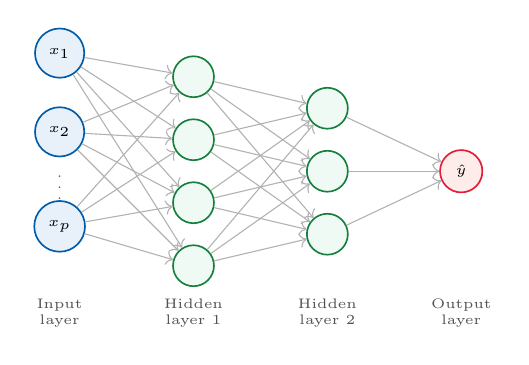
\begin{tikzpicture}[
        input/.style={circle, fill=unolightblue,  draw=unoblue,
                      line width=0.6pt, minimum size=0.52cm,
                      font=\tiny, align=center},
        hidden/.style={circle, fill=unolightgreen, draw=unogreen,
                       line width=0.6pt, minimum size=0.52cm,
                       font=\tiny, align=center},
        output/.style={circle, fill=unolightred,  draw=unored,
                       line width=0.6pt, minimum size=0.52cm,
                       font=\tiny, align=center}
      ]
        % Input layer (x=0)
        \node[input] (i1) at (0.0,  1.5) {$x_1$};
        \node[input] (i2) at (0.0,  0.5) {$x_2$};
        \node[font=\tiny, unogray] at (0.0, -0.1) {$\vdots$};
        \node[input] (i3) at (0.0, -0.7) {$x_p$};
        % Hidden layer 1 (x=1.7)
        \node[hidden] (h11) at (1.7,  1.2) {};
        \node[hidden] (h12) at (1.7,  0.4) {};
        \node[hidden] (h13) at (1.7, -0.4) {};
        \node[hidden] (h14) at (1.7, -1.2) {};
        % Hidden layer 2 (x=3.4)
        \node[hidden] (h21) at (3.4,  0.8) {};
        \node[hidden] (h22) at (3.4,  0.0) {};
        \node[hidden] (h23) at (3.4, -0.8) {};
        % Output layer (x=5.1)
        \node[output] (o1)  at (5.1,  0.0) {$\hat{y}$};
        % Connections: input -> hidden1
        \draw[gray!60, ->, line width=0.4pt] (i1) -- (h11);
        \draw[gray!60, ->, line width=0.4pt] (i1) -- (h12);
        \draw[gray!60, ->, line width=0.4pt] (i1) -- (h13);
        \draw[gray!60, ->, line width=0.4pt] (i1) -- (h14);
        \draw[gray!60, ->, line width=0.4pt] (i2) -- (h11);
        \draw[gray!60, ->, line width=0.4pt] (i2) -- (h12);
        \draw[gray!60, ->, line width=0.4pt] (i2) -- (h13);
        \draw[gray!60, ->, line width=0.4pt] (i2) -- (h14);
        \draw[gray!60, ->, line width=0.4pt] (i3) -- (h11);
        \draw[gray!60, ->, line width=0.4pt] (i3) -- (h12);
        \draw[gray!60, ->, line width=0.4pt] (i3) -- (h13);
        \draw[gray!60, ->, line width=0.4pt] (i3) -- (h14);
        % hidden1 -> hidden2
        \draw[gray!60, ->, line width=0.4pt] (h11) -- (h21);
        \draw[gray!60, ->, line width=0.4pt] (h11) -- (h22);
        \draw[gray!60, ->, line width=0.4pt] (h11) -- (h23);
        \draw[gray!60, ->, line width=0.4pt] (h12) -- (h21);
        \draw[gray!60, ->, line width=0.4pt] (h12) -- (h22);
        \draw[gray!60, ->, line width=0.4pt] (h12) -- (h23);
        \draw[gray!60, ->, line width=0.4pt] (h13) -- (h21);
        \draw[gray!60, ->, line width=0.4pt] (h13) -- (h22);
        \draw[gray!60, ->, line width=0.4pt] (h13) -- (h23);
        \draw[gray!60, ->, line width=0.4pt] (h14) -- (h21);
        \draw[gray!60, ->, line width=0.4pt] (h14) -- (h22);
        \draw[gray!60, ->, line width=0.4pt] (h14) -- (h23);
        % hidden2 -> output
        \draw[gray!60, ->, line width=0.4pt] (h21) -- (o1);
        \draw[gray!60, ->, line width=0.4pt] (h22) -- (o1);
        \draw[gray!60, ->, line width=0.4pt] (h23) -- (o1);
        % Layer labels
        \node[font=\tiny, unogray, align=center] at (0.0, -1.8)
          {Input\\layer};
        \node[font=\tiny, unogray, align=center] at (1.7, -1.8)
          {Hidden\\layer 1};
        \node[font=\tiny, unogray, align=center] at (3.4, -1.8)
          {Hidden\\layer 2};
        \node[font=\tiny, unogray, align=center] at (5.1, -1.8)
          {Output\\layer};
      \end{tikzpicture}
    \end{column}
    \begin{column}{0.46\textwidth}
      \textbf{For RSXFS forecasting:}
      \begin{itemize}
        \item \textbf{Input:} lag features $\mathbf{x}_t =
              (y_{t-1},\ldots,y_{t-12},\text{dummies})$ — a \emph{flat} vector
        \item \textbf{Hidden:} $\mathbf{h}_k = \mathrm{ReLU}(\mathbf{W}_k
              \mathbf{h}_{k-1} + \mathbf{b}_k)$ at each layer
        \item \textbf{Output:} linear (no activation) for regression
      \end{itemize}

      \medskip
      \begin{warningbox}
        \footnotesize
        A feedforward network treats its inputs as an \emph{unordered}
        feature vector. It has no notion of time order ---
        $y_{t-1}$ and $y_{t-12}$ are just two columns.
        This is why we need recurrent architectures.
      \end{warningbox}
    \end{column}
  \end{columns}
\end{frame}

% -----------------------------------------------------------------------------
\begin{frame}{Training: What the Business Analyst Needs to Know}
% -----------------------------------------------------------------------------
  \begin{columns}[T]
    \begin{column}{0.52\textwidth}
      \begin{definitionbox}{Training Loop}
        \footnotesize
        \begin{enumerate}
          \item \textbf{Forward pass:} compute predictions $\hat{y}$
          \item \textbf{Loss:} $\mathcal{L} = \mathrm{MSE}(y, \hat{y})$
          \item \textbf{Backward pass:} compute $\nabla_\mathbf{W}\mathcal{L}$
                via backpropagation
          \item \textbf{Update:} $\mathbf{W} \leftarrow
                \mathbf{W} - \eta\,\nabla_\mathbf{W}\mathcal{L}$
          \item Repeat for many epochs (passes over the training data)
        \end{enumerate}
      \end{definitionbox}

      \smallskip
      \textbf{Key hyperparameters:}
      \begin{itemize}\footnotesize
        \item Learning rate $\eta$ (Adam default: 0.001)
        \item Batch size (16--32 for small $n$)
        \item Number of epochs (use early stopping)
      \end{itemize}
    \end{column}
    \begin{column}{0.44\textwidth}
      \textit{The key practical skills are \textbf{not} deriving
      backpropagation --- they are choosing architecture depth,
      setting the learning rate, applying dropout, and recognizing
      overfitting early.}

      \medskip
      \begin{examplebox}{Adam Optimizer}
        \footnotesize
        Adam adapts the learning rate per parameter using running
        estimates of gradient mean and variance. Default
        \texttt{lr=0.001} works well for most forecasting tasks.
      \end{examplebox}
    \end{column}
  \end{columns}
\end{frame}

% =============================================================================
\section{Recurrent Neural Networks}
% =============================================================================

\sectionslide{Recurrent Neural Networks}{Sequential memory through recurrent hidden states updated at each time step}

% -----------------------------------------------------------------------------
\begin{frame}{The Vanilla RNN: Sequential Processing}
% -----------------------------------------------------------------------------
  \begin{columns}[T]
    \begin{column}{0.52\textwidth}
      \begin{definitionbox}{RNN Update Rule}
        \[
          \mathbf{h}_t = \tanh\!\bigl(
            \mathbf{W}_h \mathbf{h}_{t-1}
            + \mathbf{W}_x \mathbf{x}_t
            + \mathbf{b}
          \bigr)
        \]
        \[
          \hat{y}_{t+1} = \mathbf{w}_y^\top \mathbf{h}_t + b_y
        \]
      \end{definitionbox}

      \smallskip
      \textbf{Key properties:}
      \begin{itemize}
        \item $\mathbf{h}_t$ is a compressed summary of all past inputs
        \item $\mathbf{W}_h, \mathbf{W}_x$ are \emph{shared} across all
              time steps --- same transformation at every step
        \item $\mathbf{h}_0 = \mathbf{0}$ (no prior information at start)
      \end{itemize}
    \end{column}
    \begin{column}{0.44\textwidth}
      \begin{examplebox}{Analyst Analogy}
        \footnotesize
        An RNN reading retail sales month by month is like an analyst
        updating a running summary: each new month's number refines the
        mental model of where the trend is headed.
      \end{examplebox}

      \medskip
      \begin{warningbox}
        \footnotesize
        Shared weights mean the same transformation applies at every
        step --- efficient but limiting for very long sequences where
        patterns at very different time scales must be captured.
      \end{warningbox}
    \end{column}
  \end{columns}
\end{frame}

% -----------------------------------------------------------------------------
\begin{frame}{RNN Unrolled Through Time}
% -----------------------------------------------------------------------------
  % Unrolled RNN diagram — hardcoded coords, align=center on all nodes with \\
  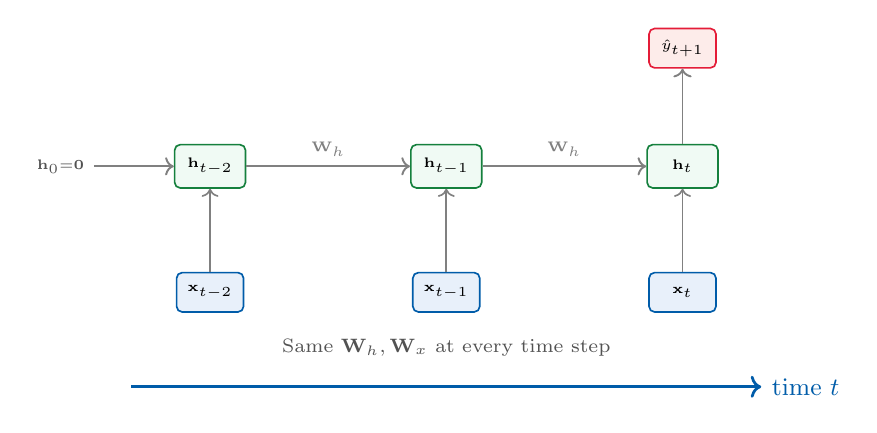
\begin{tikzpicture}[
    input/.style={rectangle, rounded corners=2pt, fill=unolightblue,
                  draw=unoblue, line width=0.6pt, minimum width=0.85cm,
                  minimum height=0.5cm, font=\tiny, align=center},
    hidden/.style={rectangle, rounded corners=2pt, fill=unolightgreen,
                   draw=unogreen, line width=0.6pt, minimum width=0.9cm,
                   minimum height=0.55cm, font=\tiny, align=center},
    output/.style={rectangle, rounded corners=2pt, fill=unolightred,
                   draw=unored, line width=0.6pt, minimum width=0.85cm,
                   minimum height=0.5cm, font=\tiny, align=center}
  ]
    % Input nodes (y=0)
    \node[input]  (x1) at (1.5, 0.0) {$\mathbf{x}_{t-2}$};
    \node[input]  (x2) at (4.5, 0.0) {$\mathbf{x}_{t-1}$};
    \node[input]  (x3) at (7.5, 0.0) {$\mathbf{x}_t$};
    % Hidden nodes (y=1.6)
    \node[hidden] (h1) at (1.5, 1.6) {$\mathbf{h}_{t-2}$};
    \node[hidden] (h2) at (4.5, 1.6) {$\mathbf{h}_{t-1}$};
    \node[hidden] (h3) at (7.5, 1.6) {$\mathbf{h}_t$};
    % Output (y=3.1)
    \node[output] (y3) at (7.5, 3.1) {$\hat{y}_{t+1}$};
    % h_0 initialisation
    \node[font=\tiny, unogray, align=center] (h0) at (-0.4, 1.6)
      {$\mathbf{h}_0{=}\mathbf{0}$};
    % Arrows: x -> h
    \draw[->, gray, line width=0.6pt] (x1) -- (h1);
    \draw[->, gray, line width=0.6pt] (x2) -- (h2);
    \draw[->, gray, line width=0.6pt] (x3) -- (h3);
    % Arrows: recurrent h_{t-1} -> h_t
    \draw[->, gray, line width=0.7pt] (h0) -- (h1);
    \draw[->, gray, line width=0.7pt] (h1) -- (h2)
      node[midway, above, font=\tiny]{$\mathbf{W}_h$};
    \draw[->, gray, line width=0.7pt] (h2) -- (h3)
      node[midway, above, font=\tiny]{$\mathbf{W}_h$};
    % Arrow: h_t -> output
    \draw[->, gray, line width=0.7pt] (h3) -- (y3);
    % "Shared weights" note
    \node[font=\scriptsize, unogray, align=center] at (4.5, -0.7)
      {Same $\mathbf{W}_h, \mathbf{W}_x$ at every time step};
    % Time arrow
    \draw[->, unoblue, line width=1.0pt] (0.5, -1.2) -- (8.5, -1.2)
      node[right, font=\small]{time $t$};
  \end{tikzpicture}

  \vspace{2pt}
  \muted{\footnotesize\itshape
    Socratic: the same $\mathbf{W}_h$ and $\mathbf{W}_x$ apply at every time step.
    What does this shared-parameter constraint imply about how the model
    treats January vs.\ July?}
\end{frame}

% -----------------------------------------------------------------------------
\begin{frame}{Why Vanilla RNNs Fail on Long Sequences}
% -----------------------------------------------------------------------------
  \begin{columns}[T]
    \begin{column}{0.54\textwidth}
      \begin{definitionbox}{Vanishing Gradient}
        \footnotesize\muted{\footnotesize\parencite{Bengio1994}}\\[-4pt]
        Backpropagating through $T$ steps requires multiplying $T$ copies
        of $\mathbf{W}_h^\top$:
        \vspace{-4pt}
        \[
          \frac{\partial \mathcal{L}}{\partial \mathbf{h}_0}
          \propto \bigl(\mathbf{W}_h^\top\bigr)^T
        \]
        \vspace{-6pt}
        If $|\lambda_{\max}(\mathbf{W}_h)| < 1$, this product $\to \mathbf{0}$
        exponentially. Weights early in the sequence receive
        near-zero gradients --- the model \emph{forgets} the distant past.
      \end{definitionbox}
      \muted{\tiny $\lambda_{\max}$ = spectral radius of $\mathbf{W}_h$;
        unrelated to regularization $\lambda$ from Lecture 08.}

      \vspace{2pt}
      \textbf{Consequences for forecasting:}
      \begin{itemize}
        \item A vanilla RNN trained on RSXFS cannot reliably learn that
              December sales are high because \emph{December was high 12
              months ago}
        \item The 12-month seasonal dependency is precisely where
              vanilla RNNs fail
      \end{itemize}
    \end{column}
    \begin{column}{0.42\textwidth}
      \begin{warningbox}
        Vanilla RNNs work for 5--10 step dependencies.
        For monthly seasonality (lag 12) or multi-year cycles,
        they systematically underperform.
      \end{warningbox}

      \smallskip
      \textit{\footnotesize
        The fix: LSTM introduces gating mechanisms that
        protect long-range gradients by creating a direct
        \emph{information highway} across time steps.}
    \end{column}
  \end{columns}

\end{frame}

% =============================================================================
\section{LSTM: Long Short-Term Memory}
% =============================================================================

\sectionslide{LSTM: Long Short-Term Memory}{Gated cell state solves the vanishing gradient problem for long-range dependencies}

% -----------------------------------------------------------------------------
\begin{frame}{LSTM Gates: Forget, Input, Output}
% -----------------------------------------------------------------------------
  \begin{columns}[T]
    \begin{column}{0.56\textwidth}
      \begin{definitionbox}{LSTM Gate Equations}
        \footnotesize\muted{\footnotesize\parencite{Hochreiter1997}}
        Here $[\mathbf{h}_{t-1},\,\mathbf{x}_t]$ denotes horizontal concatenation.
        $\sigma$ = sigmoid (here specifically); $\odot$ = element-wise product.
        \vspace{-2pt}
        \begin{align*}
          f_t &= \sigma(\mathbf{W}_f [\mathbf{h}_{t-1},\,\mathbf{x}_t]
                 + \mathbf{b}_f)
                 \quad\text{(forget)}\\
          i_t &= \sigma(\mathbf{W}_i [\mathbf{h}_{t-1},\,\mathbf{x}_t]
                 + \mathbf{b}_i)
                 \quad\text{(input)}\\
          \tilde{\mathbf{c}}_t &= \tanh(\mathbf{W}_g [\mathbf{h}_{t-1},\,\mathbf{x}_t]
                 + \mathbf{b}_g)
                 \quad\text{(candidate)}\\
          o_t &= \sigma(\mathbf{W}_o [\mathbf{h}_{t-1},\,\mathbf{x}_t]
                 + \mathbf{b}_o)
                 \quad\text{(output)}\\[2pt]
          \mathbf{c}_t &= f_t \odot \mathbf{c}_{t-1}
                 + i_t \odot \tilde{\mathbf{c}}_t\\
          \mathbf{h}_t &= o_t \odot \tanh(\mathbf{c}_t)
        \end{align*}
        Gates $f_t, i_t, o_t \in (0,1)^d$ are \emph{vectors}; $\mathbf{h}_{t-1}$ and $\mathbf{x}_t$ were defined in the RNN section.
        \muted{\footnotesize\itshape (Cell data flow on next slide.)}
      \end{definitionbox}
    \end{column}
    \begin{column}{0.40\textwidth}
      \footnotesize
      \textbf{Forget gate $f_t$:}
      \textit{$f_t \approx 1$: keep memory; $f_t \approx 0$: erase.
      During a recession, the model learns to reset the normal-growth signal.}

      \medskip
      \textbf{Input gate $i_t$:}
      \textit{Controls which new information enters cell state.
      A large December dummy triggers high $i_t$ to write the holiday pattern.}

      \medskip
      \textbf{Output gate $o_t$:}
      \textit{Controls which part of cell state flows to $\mathbf{h}_t$
      --- what is announced to the next layer.}
    \end{column}
  \end{columns}
\end{frame}

% -----------------------------------------------------------------------------
\begin{frame}{LSTM Cell Architecture}
% -----------------------------------------------------------------------------
  % LSTM cell diagram — hardcoded coords, align=center on all multi-line nodes
  \begin{center}
  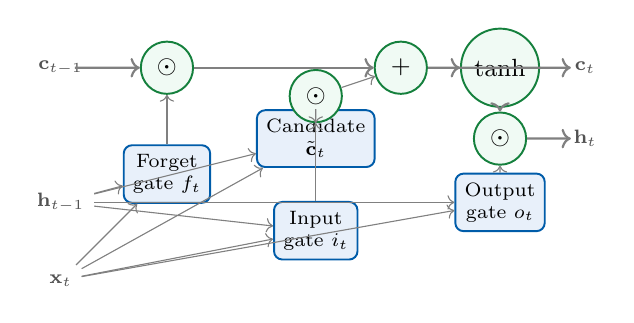
\begin{tikzpicture}[xscale=0.90, yscale=0.90,
    gate/.style={rectangle, rounded corners=3pt, fill=unolightblue,
                 draw=unoblue, line width=0.7pt, minimum width=1.0cm,
                 minimum height=0.52cm, font=\scriptsize, align=center},
    op/.style={circle, fill=unolightgreen, draw=unogreen,
               line width=0.7pt, minimum size=0.42cm,
               font=\small, align=center}
  ]
    % Cell state highway (top)
    \node[font=\scriptsize, unogray] at (-0.2, 3.5) {$\mathbf{c}_{t-1}$};
    \node[font=\scriptsize, unogray] at (7.2,  3.5) {$\mathbf{c}_t$};
    % Forget gate
    \node[gate] (fg)    at (1.3, 2.0) {Forget\\gate $f_t$};
    % Multiply: c_{t-1} * f_t
    \node[op]   (mul1)  at (1.3, 3.5) {$\odot$};
    % Input gate + candidate
    \node[gate] (ig)    at (3.4, 1.2) {Input\\gate $i_t$};
    \node[gate] (cand)  at (3.4, 2.5) {Candidate\\$\tilde{\mathbf{c}}_t$};
    % Multiply: i_t * c_tilde
    \node[op]   (mul2)  at (3.4, 3.1) {$\odot$};
    % Add: new cell state
    \node[op]   (add1)  at (4.6, 3.5) {$+$};
    % Output gate
    \node[gate] (og)    at (6.0, 1.6) {Output\\gate $o_t$};
    % tanh of new cell
    \node[op]   (tanh1) at (6.0, 3.5) {tanh};
    % Multiply: o_t * tanh(c_t)
    \node[op]   (mul3)  at (6.0, 2.5) {$\odot$};
    % Inputs (left)
    \node[font=\scriptsize, unogray] (hin) at (-0.2, 1.6)
      {$\mathbf{h}_{t-1}$};
    \node[font=\scriptsize, unogray] (xin) at (-0.2, 0.5)
      {$\mathbf{x}_t$};
    % Output (right)
    \node[font=\scriptsize, unogray] (hout) at (7.2, 2.5)
      {$\mathbf{h}_t$};

    % Cell state highway connections
    \draw[->, gray, line width=0.8pt] (-0.0, 3.5) -- (mul1);
    \draw[->, gray, line width=0.8pt] (mul1) -- (add1);
    \draw[->, gray, line width=0.8pt] (add1) -- (tanh1);
    \draw[->, gray, line width=0.8pt] (tanh1) -- (mul3);
    \draw[->, gray, line width=0.8pt] (mul3) -- (7.0, 2.5);
    % c_t continues right
    \draw[->, gray, line width=0.8pt] (add1) -- (7.0, 3.5);

    % Forget gate connections
    \draw[->, gray] (hin) -- (fg);
    \draw[->, gray] (xin) -- (fg);
    \draw[->, gray] (fg)  -- (mul1);

    % Input gate + candidate -> mul2
    \draw[->, gray] (hin)  -- (ig);
    \draw[->, gray] (xin)  -- (ig);
    \draw[->, gray] (hin)  -- (cand);
    \draw[->, gray] (xin)  -- (cand);
    \draw[->, gray] (ig)   -- (mul2);
    \draw[->, gray] (cand) -- (mul2);
    \draw[->, gray] (mul2) -- (add1);

    % Output gate connections
    \draw[->, gray] (hin) -- (og);
    \draw[->, gray] (xin) -- (og);
    \draw[->, gray] (og)  -- (mul3);
  \end{tikzpicture}
  \end{center}

  \vspace{-2pt}
  \begin{keybox}
    \footnotesize
    The cell state $\mathbf{c}_t$ flows through with only $\odot$ and $+$
    operations --- gradients can propagate back without shrinking to zero.
  \end{keybox}
\end{frame}

% -----------------------------------------------------------------------------
\begin{frame}{LSTM for Time Series: Practical Setup}
% -----------------------------------------------------------------------------
  \begin{columns}[T]
    \begin{column}{0.52\textwidth}
      \begin{definitionbox}{LSTM Forecasting Setup}
        \footnotesize
        \begin{enumerate}
          \item \textbf{Reshape:} stack $T$ consecutive feature vectors into
                a 3-D array: $(\mathbf{x}_{t-T+1}, \ldots, \mathbf{x}_t)$
          \item \textbf{Process:} LSTM updates $\mathbf{h}_s, \mathbf{c}_s$
                at each step $s = t-T+1, \ldots, t$
          \item \textbf{Predict:} pass final $\mathbf{h}_t$ to a Dense
                layer: $\hat{y}_{t+1} = \mathbf{w}^\top \mathbf{h}_t + b$
        \end{enumerate}
        Lookback window $T$ is the key design choice.
      \end{definitionbox}

      \smallskip
      \textbf{Architecture options:}
      \begin{itemize}\footnotesize
        \item \textbf{Single LSTM layer:} short-run patterns
        \item \textbf{Stacked (2-layer) LSTM:} first = momentum,
              second = seasonal structure; often best for monthly data
      \end{itemize}
    \end{column}
    \begin{column}{0.44\textwidth}
      \begin{keybox}
        \footnotesize
        For RSXFS with strong 12-month seasonality, use
        $T \geq 24$ (two full years) to give the LSTM enough
        context to learn the annual pattern.
      \end{keybox}

      \smallskip
      \textit{\footnotesize Note: the first $T$ observations are consumed
      to build the initial sequence and cannot serve as targets. With
      $T = 24$, document this 24-month shift when reporting sample sizes.}
    \end{column}
  \end{columns}
\end{frame}

% -----------------------------------------------------------------------------
\begin{frame}{LSTM Key Hyperparameters}
% -----------------------------------------------------------------------------
  \begin{center}
  \footnotesize
  \begin{tabular}{p{2.6cm}p{2.8cm}p{1.6cm}p{4.0cm}}
    \toprule
    \textbf{Parameter} & \textbf{Keras name} & \textbf{Typical} & \textbf{Effect} \\
    \midrule
    Lookback window
      & \texttt{T} (manual reshape)
      & 24--36
      & Longer = more seasonal context; larger model \\
    LSTM units
      & \texttt{units}
      & 32--128
      & More = higher capacity; overfit risk \\
    LSTM layers
      & (stack 2)
      & 1--2
      & Second layer captures longer patterns \\
    Dropout
      & \texttt{dropout,} \texttt{recurrent\_dropout}
      & 0.1--0.3
      & Regularization; crucial for small $n$ \\
    Learning rate
      & \texttt{lr} (Adam)
      & 0.001
      & Default works; reduce if training unstable \\
    Epochs
      & \texttt{epochs}
      & 50--200
      & Use \texttt{EarlyStopping(patience=20)} \\
    \bottomrule
  \end{tabular}
  \end{center}

  \medskip
  \begin{keybox}
    \footnotesize
    With $n \approx 300$ monthly observations, LSTM is
    \emph{data-limited}. Use small units (32--64), dropout ($\geq$ 0.2),
    and \texttt{EarlyStopping}. Larger capacity will overfit.
    Run 5 random seeds; report median RMSE.
  \end{keybox}

  \muted{\footnotesize\itshape
    Socratic: LSTM dropout ($\geq$ 0.2) regularizes similarly to LASSO from Lecture 08.
    What is the key conceptual difference between dropout-based regularization
    and L1 penalty-based regularization (LASSO)?}
\end{frame}

% =============================================================================
\section{Attention Mechanisms}
% =============================================================================

\sectionslide{Attention Mechanisms}{Direct access to any past time step without sequential compression}

% -----------------------------------------------------------------------------
\begin{frame}{Attention: What the Model Learns to Focus On}
% -----------------------------------------------------------------------------
  \begin{center}
  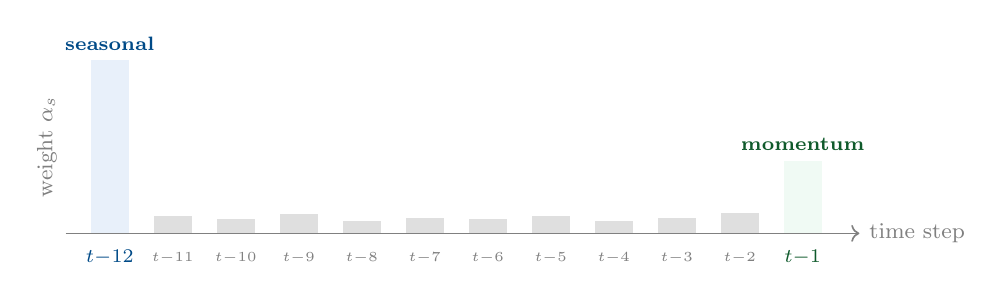
\begin{tikzpicture}[xscale=0.80, yscale=2.2]
    % Bars: attention weights for steps t-12 through t-1
    % t-12 = seasonal spike (UNO blue), t-1 = momentum (UNO green), others gray
    \fill[unolightblue]    (0.3,0) rectangle (0.9,1.0);
    \fill[gray!25] (1.3,0) rectangle (1.9,0.10);
    \fill[gray!25] (2.3,0) rectangle (2.9,0.08);
    \fill[gray!25] (3.3,0) rectangle (3.9,0.11);
    \fill[gray!25] (4.3,0) rectangle (4.9,0.07);
    \fill[gray!25] (5.3,0) rectangle (5.9,0.09);
    \fill[gray!25] (6.3,0) rectangle (6.9,0.08);
    \fill[gray!25] (7.3,0) rectangle (7.9,0.10);
    \fill[gray!25] (8.3,0) rectangle (8.9,0.07);
    \fill[gray!25] (9.3,0) rectangle (9.9,0.09);
    \fill[gray!25](10.3,0) rectangle (10.9,0.12);
    \fill[unolightgreen]  (11.3,0) rectangle (11.9,0.42);
    % x-axis
    \draw[->, gray, line width=0.6pt] (-0.1,0) -- (12.5,0)
          node[right, font=\footnotesize, gray] {time step};
    % x-axis labels (explicit — no \foreach)
    \node[font=\scriptsize, text=unoblue!80!black] at  (0.6,-0.14) {$t{-}12$};
    \node[font=\tiny, text=gray]                   at  (1.6,-0.14) {$t{-}11$};
    \node[font=\tiny, text=gray]                   at  (2.6,-0.14) {$t{-}10$};
    \node[font=\tiny, text=gray]                   at  (3.6,-0.14) {$t{-}9$};
    \node[font=\tiny, text=gray]                   at  (4.6,-0.14) {$t{-}8$};
    \node[font=\tiny, text=gray]                   at  (5.6,-0.14) {$t{-}7$};
    \node[font=\tiny, text=gray]                   at  (6.6,-0.14) {$t{-}6$};
    \node[font=\tiny, text=gray]                   at  (7.6,-0.14) {$t{-}5$};
    \node[font=\tiny, text=gray]                   at  (8.6,-0.14) {$t{-}4$};
    \node[font=\tiny, text=gray]                   at  (9.6,-0.14) {$t{-}3$};
    \node[font=\tiny, text=gray]                   at (10.6,-0.14) {$t{-}2$};
    \node[font=\scriptsize, text=unogreen!70!black] at (11.6,-0.14) {$t{-}1$};
    % y-axis label
    \node[font=\footnotesize, rotate=90, text=gray] at (-0.4,0.5) {weight $\alpha_s$};
    % annotations
    \node[font=\scriptsize, text=unoblue!80!black, above] at (0.6,1.0)
          {\textbf{seasonal}};
    \node[font=\scriptsize, text=unogreen!70!black, above] at (11.6,0.42)
          {\textbf{momentum}};
  \end{tikzpicture}
  \end{center}

  \begin{itemize}\footnotesize
    \item \textbf{High weight at $t-12$:} attending to ``same month last year'' ---
          an LSTM must propagate this 12 steps; attention reads it \emph{directly}
    \item \textbf{Medium weight at $t-1$:} short-run momentum
    \item \textbf{Near-zero elsewhere:} the model ignores irrelevant lags ---
          no manual feature engineering required
  \end{itemize}
\end{frame}

% -----------------------------------------------------------------------------
\begin{frame}{Attention: Formal Definition}
% -----------------------------------------------------------------------------
  \begin{columns}[T]
    \begin{column}{0.52\textwidth}
      \begin{definitionbox}{Scaled Dot-Product Attention (simplified)}
        \footnotesize
        Let $\mathbf{H} = [\mathbf{h}_1, \ldots, \mathbf{h}_T]$ be the stacked
        hidden states and $\mathbf{q}$ the query at the current step:
        \[
          \boldsymbol{\alpha}
          = \mathrm{softmax}\!\left(
              \frac{\mathbf{H}\mathbf{q}}{\sqrt{d_k}}
            \right),
          \quad
          \mathrm{context} = \mathbf{H}^\top \boldsymbol{\alpha}
        \]
        $d_k$ = key-vector dimension; $\sqrt{d_k}$ prevents the dot product
        from growing large and saturating the softmax.
        Weights $\boldsymbol{\alpha} = (\alpha_1,\ldots,\alpha_T)^\top$ sum to 1
        (one scalar $\alpha_s$ per time step) and are learned end-to-end.
      \end{definitionbox}

      \smallskip
      \muted{\footnotesize\itshape
        Simplified single-query form; \textcite{Vaswani2017} use a full
        multi-head $(\mathbf{Q},\mathbf{K},\mathbf{V})$ formulation.}

      \vspace{3pt}
      \muted{\footnotesize\itshape
        Note: $\boldsymbol{\alpha}$ here denotes attention weights ---
        distinct from ETS smoothing $\alpha$ (L03), ECM adjustment $\alpha$
        (L05), and Elastic Net mixing $\alpha$ (L08).}
    \end{column}
    \begin{column}{0.44\textwidth}
      \begin{examplebox}{What Attention Solves}
        \footnotesize
        In LSTM, information at step $t-12$ must survive 12 hidden-state
        updates and can get diluted. Attention \emph{directly} reads
        $\mathbf{h}_{t-12}$ with weight $\alpha_{t-12}$ ---
        no intermediate compression.
      \end{examplebox}
    \end{column}
  \end{columns}
\end{frame}

% -----------------------------------------------------------------------------
\begin{frame}{Transformers and Practical Guidance}
% -----------------------------------------------------------------------------
  \textbf{The Transformer \parencite{Vaswani2017}:}
  \begin{itemize}
    \item Originally designed for NLP (language translation)
    \item Replaces recurrence entirely with \emph{multi-head self-attention}
    \item Parallelizes perfectly over time steps --- no sequential bottleneck
    \item Requires substantially more data than LSTM to train well
  \end{itemize}

  \medskip
  \begin{keybox}
    \textbf{Practical guidance for business forecasting:}
    \begin{itemize}
      \item Monthly data, $n \approx 300$: Transformer is over-parameterized;
            LSTM $\pm$ attention is the practical sweet spot
      \item Daily/weekly data, $n > 5{,}000$: Transformer or
            Temporal Fusion Transformer (TFT) is state-of-the-art
      \item Multi-series panel ($N$ stores $\times$ $T$ months):
            train one LSTM/Transformer on all series simultaneously
    \end{itemize}
  \end{keybox}

  \medskip
  \muted{\footnotesize\itshape
    Socratic: self-attention treats its inputs as an unordered set of vectors ---
    it has no built-in notion of sequence position.
    Why is \emph{positional encoding} essential for Transformers?}
\end{frame}

% =============================================================================
\section{Keras Implementation}
% =============================================================================

\sectionslide{Keras Implementation}{Two-layer LSTM for business forecasting with sequence reshaping}

% -----------------------------------------------------------------------------
\begin{frame}[fragile]{LSTM in Keras: Minimal Working Example}
% -----------------------------------------------------------------------------
  \begin{columns}[T]
    \begin{column}{0.49\textwidth}
      \textbf{Step 1: Build sequences}
\begin{lstlisting}[language=Python, basicstyle=\tiny\ttfamily]
import numpy as np
from tensorflow import keras
from tensorflow.keras import layers

T = 24  # lookback window (months)

def make_sequences(X_arr, y_arr, T):
    """Reshape to (n_samples, T, n_features)."""
    Xs, ys = [], []
    for i in range(T, len(X_arr)):
        Xs.append(X_arr[i-T:i])
        ys.append(y_arr[i])
    return np.array(Xs), np.array(ys)

X_arr = X.values.astype('float32')
y_arr = y.values.astype('float32')
Xs, ys = make_sequences(X_arr, y_arr, T)

# Chronological split (no shuffling)
n = len(ys)
n_test = int(0.15 * n)
n_val  = int(0.15 * n)
Xs_tr = Xs[:n-n_test-n_val]
ys_tr = ys[:n-n_test-n_val]
Xs_va = Xs[n-n_test-n_val:n-n_test]
ys_va = ys[n-n_test-n_val:n-n_test]
Xs_te = Xs[n-n_test:]
ys_te = ys[n-n_test:]
\end{lstlisting}
    \end{column}
    \begin{column}{0.48\textwidth}
      \textbf{Step 2: Build and train}
\begin{lstlisting}[language=Python, basicstyle=\tiny\ttfamily]
n_features = Xs_tr.shape[2]

model = keras.Sequential([
    layers.LSTM(64,
        return_sequences=True,
        dropout=0.2,
        recurrent_dropout=0.1,
        input_shape=(T, n_features)),
    layers.LSTM(32, dropout=0.2),
    layers.Dense(1)
])
model.compile(
    optimizer=keras.optimizers.Adam(learning_rate=0.001),
    loss='mse')

cb = keras.callbacks.EarlyStopping(
    patience=20,
    restore_best_weights=True)

history = model.fit(
    Xs_tr, ys_tr,
    validation_data=(Xs_va, ys_va),
    epochs=200,
    batch_size=16,
    callbacks=[cb],
    verbose=0)

y_pred = model.predict(Xs_te).flatten()
\end{lstlisting}
    \end{column}
  \end{columns}
\end{frame}

% =============================================================================
\section{Application to Forecasting}
% =============================================================================

\sectionslide{Application to Forecasting}{Comparing LSTM against the full Lectures 01--09 leaderboard on RSXFS}

% -----------------------------------------------------------------------------
\begin{frame}{When Does LSTM Help? Data Requirements}
% -----------------------------------------------------------------------------
  \begin{columns}[T]
    \begin{column}{0.52\textwidth}
      \begin{warningbox}
        \textbf{LSTM vs.\ XGBoost on small datasets:}
        A two-layer LSTM with 64 units has ${\approx}\,50{,}000$ parameters.
        XGBoost with 500 trees and depth 4 is sparse by comparison.
        With $n \approx 300$, this is a fundamental
        parameter-to-data mismatch.
      \end{warningbox}

      \medskip
      \textbf{Rule of thumb:}
      \begin{itemize}
        \item $n < 500$ monthly: XGBoost wins (more reproducible)
        \item $n > 1{,}000$ daily/weekly: LSTM competitive
        \item $N$ series $\times$ $T$ months (panel): LSTM scales well
        \item Long-range patterns beyond 12 months: LSTM advantage
              grows
      \end{itemize}
    \end{column}
    \begin{column}{0.44\textwidth}
      \begin{examplebox}{When LSTM Wins}
        \begin{itemize}
          \item Daily energy demand or stock prices ($n > 3{,}000$)
          \item Multi-store retail panel: one LSTM across 1,000 stores
          \item Sequences with multi-scale patterns not captured by
                a fixed lag window
        \end{itemize}
      \end{examplebox}

      \medskip
      \muted{\footnotesize\itshape
        On RSXFS alone ($n \approx 300$), expect LSTM RMSE
        $\approx$ 2{,}100--2{,}600 across seeds. The median is competitive
        with XGBoost but with higher variance. Always report median
        over $\geq 5$ seeds.}
    \end{column}
  \end{columns}
\end{frame}

% -----------------------------------------------------------------------------
\begin{frame}{Full Model Leaderboard: Lectures 01--10}
% -----------------------------------------------------------------------------
  \begin{columns}[T]
    \begin{column}{0.52\textwidth}
      \textbf{Test-set results on RSXFS (24-month horizon):}
      \begin{center}
      \footnotesize
      \begin{tabular}{lrr}
        \toprule
        \textbf{Model} & \textbf{RMSE} & \textbf{MAE} \\
        \midrule
        Seasonal Na\"{i}ve             & 4\,210 & 3\,120 \\
        SARIMA(1,1,1)(1,1,1)$_{12}$    & 2\,840 & 2\,100 \\
        Elastic Net ($\lambda^*$)      & 2\,540 & 1\,890 \\
        Random Forest                  & 2\,380 & 1\,760 \\
        XGBoost (early stop)           & 2\,250 & 1\,650 \\
        LSTM (2-layer, $T\!=\!24$)     & 2\,180 & 1\,600 \\
        \bottomrule
      \end{tabular}
      \end{center}
      \muted{\footnotesize\itshape
        Values are illustrative. LSTM = median over 5 seeds.
        Strategy: direct multi-step (one model per horizon).}
    \end{column}
    \begin{column}{0.44\textwidth}
      \textbf{Interpretation:}
      \begin{itemize}
        \item LSTM edges XGBoost by $\sim$70 RMSE --- a modest,
              seed-sensitive improvement
        \item XGBoost is more \emph{reproducible} (deterministic at
              \texttt{random\_state=42}); LSTM requires seed averaging
        \item Both require feature engineering; LSTM additionally
              needs sequence reshaping
      \end{itemize}

      \medskip
      \begin{keybox}
        \footnotesize
        XGBoost remains the recommended default for monthly macro data.
        Use LSTM when you have daily data, panel data across many
        series, or need to capture complex multi-scale temporal patterns.
      \end{keybox}
    \end{column}
  \end{columns}
\end{frame}

% =============================================================================
\section{Takeaways and References}
% =============================================================================

\sectionslide{Takeaways and References}{What we learned and where to go next}

% -----------------------------------------------------------------------------
\begin{frame}{Lecture 10 Key Takeaways}
% -----------------------------------------------------------------------------
  \begin{keybox}
    \footnotesize
    \begin{enumerate}
      \item \textbf{Feedforward networks} are universal approximators but
            treat inputs as unordered feature vectors --- no built-in
            time awareness.
      \item \textbf{Vanilla RNNs} add sequential memory but suffer
            vanishing gradients \parencite{Bengio1994} --- reliable only
            for dependencies $\leq 5$--10 steps back.
      \item \textbf{LSTM} \parencite{Hochreiter1997} solves this with
            three gates (forget, input, output) and a protected cell state
            that carries information over long sequences.
      \item \textbf{Attention} \parencite{Vaswani2017} lets the model
            directly weight any past time step. Transformers generalize
            this but require far more data.
      \item \textbf{Data size is the key constraint:} on $n \approx 300$
            monthly obs., LSTM's margin over XGBoost is narrow and
            seed-sensitive. Always report median over $\geq 5$ seeds.
      \item \textbf{Practical rule:} use XGBoost as your default ML
            forecaster for monthly macro data; use LSTM when you have
            daily/weekly data, panel data, or multi-step horizons with
            long-range dependencies.
    \end{enumerate}
  \end{keybox}

  \smallskip
  \textbf{Preview of Lecture 11:} Feature Engineering ---
  lags, rolling statistics, calendar effects, and pipeline design for
  both tree-based and neural network forecasters.
\end{frame}

% -----------------------------------------------------------------------------
\begin{frame}{References}
% -----------------------------------------------------------------------------
  \printbibliography[heading=none]
\end{frame}

% =============================================================================
\end{document}
% =============================================================================
